\chapter{Pruebas y Resultados}
\label{cap:7}

En el presente capítulo se describen las pruebas de campo y los resultados obtenidos. El primer grupo de pruebas tuvo por objetivo determinar los valores más adecuados para los parámetros utilizados en la recolección de FCD, tanto en el reconocimiento de actividad como en la toma de localizaciones. Las demás pruebas se realizaron con el objetivo determinar la efectividad del sistema implementado, para ello se verificó la tasa de acierto del algoritmo de MM y se analizaron los datos obtenidos mediante la estimación de tráfico.

Para las pruebas se utilizaron dispositivos móviles de diversa gama y se realizaron tanto en vehículos de transporte público, como en automóviles. La mayoría de las pruebas fueron realizadas en días laborales. Debido a la complejidad y a la gran cantidad de variables intervinientes en el funcionamiento del sistema se optó por realizar pruebas de campo y no utilizar ninguna simulación.

\section{Floating Car Data}

Para la obtención de FCD se utiliza un esquema de detección de actividad que permite a la aplicación registrar las localizaciones del usuario únicamente cuando se encuentra en un vehículo en movimiento. Para ello, la aplicación móvil verifica periódicamente cuál es la actividad que está realizando el usuario en base a las lecturas de los sensores del dispositivo. El intervalo de tiempo en el que se realiza esta verificación se denomina \emph{intervalo de reconocimiento} y determina qué tan rápido se detecta el movimiento y se inicia el rastreo. La \Cref{tab:prom_intervalo_reconocimiento} muestra el tiempo promedio que la aplicación tarda en detectar el movimiento e iniciar la toma de localizaciones para varios valores del intervalo de reconocimiento. Como se puede apreciar, un intervalo de reconocimiento corto ayuda a iniciar más rápidamente la toma de localizaciones. Es importante tener en cuenta que mientras más corto es el intervalo, mayor es el consumo de batería debido a que el dispositivo móvil debe procesar más frecuentemente las muestras de los sensores.

\begin{table}[h]
  \centering
	\begin{tabular}{cccc}
	\toprule
	Intervalo (s) & En bus (min.) & En auto (min.) & Ambos (min.) \\
	\midrule
	15            & 2.83         & 1.25          & 2.43           \\
	30            & 1.43         & 1.75          & 1.54           \\
	60            & 5.5          & 2.75          & 4.4            \\
	\bottomrule
	\end{tabular}
  \caption{Tiempos promedio para inicio de rastreo}
  \label{tab:prom_intervalo_reconocimiento}
\end{table}

En base a las pruebas realizadas se seleccionó un intervalo de reconocimiento de 30 segundos por ser el intervalo más largo que aún da tiempos de respuesta aceptables para el inicio de la toma de localizaciones.

El reconocimiento de actividad también es utilizado para detener la toma de localizaciones cuando el usuario ya no se encuentra en un vehículo en movimiento. Un problema ocurre cuando durante una trayectoria el vehículo deja de estar en movimiento debido a diversas causas, como ser un semáforo en rojo o una parada de bus. En estos casos la toma de localizaciones puede ser erróneamente detenida, lo que produce cortes en el trayecto recorrido. Para evitar estos cortes se introduce un \emph{tiempo de tolerancia} en el reconocimiento de actividad. Cada vez que se detecta el movimiento, se almacena el tiempo de detección y el rastreo no es detenido hasta que haya transcurrido el tiempo de tolerancia a partir de la última detección de movimiento. El porcentaje de tiempo que el dispositivo estuvo rastreando al usuario con respecto al tiempo total que duró el viaje se denomina \emph{tiempo efectivo de rastreo}. El objetivo es evitar cortes durante el trayecto del usuario, de manera a maximizar el tiempo efectivo de rastreo. El tiempo de tolerancia, en combinación con el intervalo de reconocimiento, influyen en el tiempo efectivo de rastreo. Un tiempo de tolerancia alto implica que se tardará más en detener el servicio de localización, lo que puede producir un impacto negativo en el consumo de batería.

\begin{table}[h]
  \centering
	\begin{tabular}{ccccc}
	\toprule
	Intervalo (s) & Tolerancia (min.) & En bus (min.) & En auto (min.) & Ambos (min.) \\
	\midrule
	15            & 5                 & 84.86         & 84.86          & 84.86        \\
	30            & 5                 & 89.31         & 89.31          & 89.31        \\
	60            & 5                 & 80.83         & 80.83          & 80.83        \\
	15            & 10                & 94.44         & 94.44          & 94.44        \\
	30            & 10                & 95.83         & 95.83          & 95.83        \\
	60            & 10                & 83.33         & 83.33          & 83.33        \\
	\bottomrule
	\end{tabular}
  \caption{Tiempos efectivos de rastreo}
  \label{tab:prom_tiempo_efectivo_rastreo}
\end{table}

La \Cref{tab:prom_tiempo_efectivo_rastreo} muestra los valores para el porcentaje del tiempo efectivo de rastreo para cada combinación de intervalo de reconocimiento y toma de localizaciones. Una tolerancia de 10 minutos combinada con un intervalo de reconocimiento de 30 segundos produce los mejores resultados en el estudio de campo realizado.

\section{Map Matching}

Para el Map Matching se utiliza el algoritmo ST-Matching como se describe en \cref{implementacion_mm}. Este algoritmo recibe como entrada un conjunto de localizaciones correspondientes a una ruta seguida por un usuario, el intervalo de tiempo con el que se obtienen estos puntos se denomina \emph{frecuencia de muestreo}. Si esta frecuencia es baja, se tiene un menor número de muestras para un periodo de tiempo dado y un menor consumo de batería por parte del teléfono móvil. En cambio par frecuencias altas, se tiene un mayor número de muestras así como un elevado consumo de batería. Para medir la efectividad del MM, se observa la cantidad de aciertos del mismo al estimar una ruta.

Las pruebas sobre el MM consistieron en la observación de su efectividad con diferentes \emph{frecuencias de muestreo}. Las frecuencias observadas fueron de 2, 1 y 0.5 localizaciones por minuto, que corresponden a intervalos de tiempo de 30, 60 y 120 segundos respectivamente entre una ubicación y otra. las pruebas realizadas, se definieron  tres frecuencias para la toma de localizaciones: 30, 60 y 120 segundos. 

\begin{table}[ht]
	\caption{Efectividad del MM} 
	\centering
	\begin{tabular}{c c c c}
		\hline\hline
		Intervalo (s) & Total de Puntos & Puntos Correctos & Porcentaje de Acierto\\ [0.5ex]
		\hline
		30 & 80 & 74 & 92 \\
		60 & 100 & 91 & 91 \\
		120 & 83 & 73 & 88\\ [1ex]
		\hline
	\end{tabular}
	\label{table:map_matching}
\end{table}

En la tabla \ref{table:map_matching} se pueden apreciar los resultados obtenidos. Para intervalos pequeños de toma localizaciones  se tienen mejores resultados, con una diferencia a favor del intervalo de 30 segundos de 1\% en comparación a 60 segundos y de 4\% en comparación a 120 segundos.  

A continuación se presenta el desempeño del MM para un mismo recorrido utilizando las tres frecuencias analizadas. Se muestra con una línea roja el recorrido observado por el vehículo, y con una línea verde el recorrido aproximado después de realizar el MM. La \cref{fig:mm_30s} corresponde a las muestras obtenidas utilizando un intervalo de muestreo de 20 segundos, las figuras \ref{fig:mm_1m} y \ref{fig:mm_2m} corresponden a intervalos de 1 y 2 minutos respectivamente. Se puede observar que con intervalos separados de tiempo, las localizaciones tomadas están más distanciadas entre si. Gracias al algoritmo de MM utilizado, el camino generado es práctiacmente el mismo para las frecuencias observadas.

\begin{figure}[!htb]
	\centering
	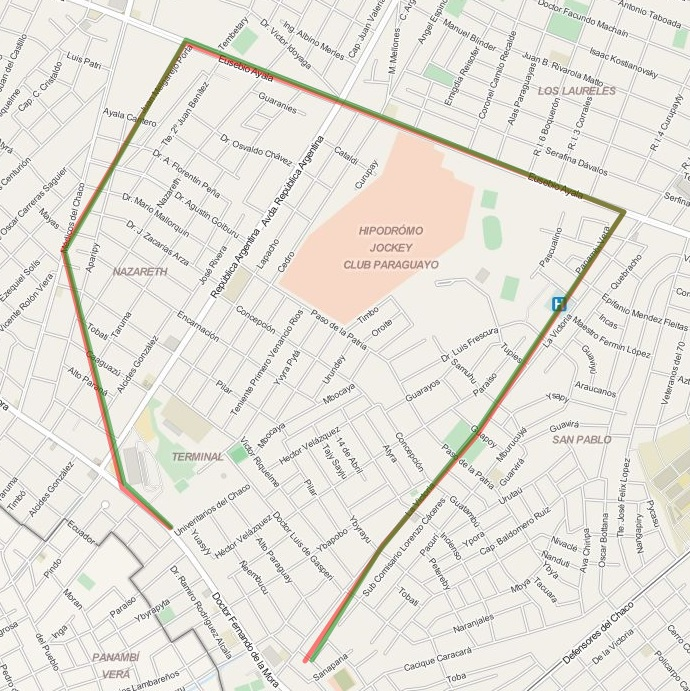
\includegraphics[width=0.7\textwidth]{capitulos/7/figuras/figura1.jpg}
	\caption{\label{fig:mm_30s} MM con intervalo de 30 segundos}	
\end{figure}

\begin{figure}[!htb]
	\centering
	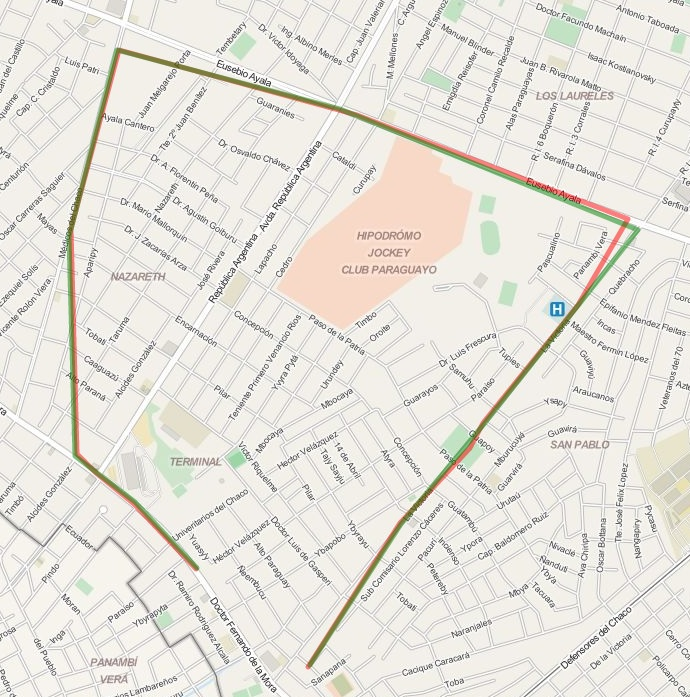
\includegraphics[width=0.7\textwidth]{capitulos/7/figuras/figura2.jpg}
	\caption{\label{fig:mm_1m} MM con intervalo de 1 minuto}	
\end{figure}

\begin{figure}[!htb]
	\centering
	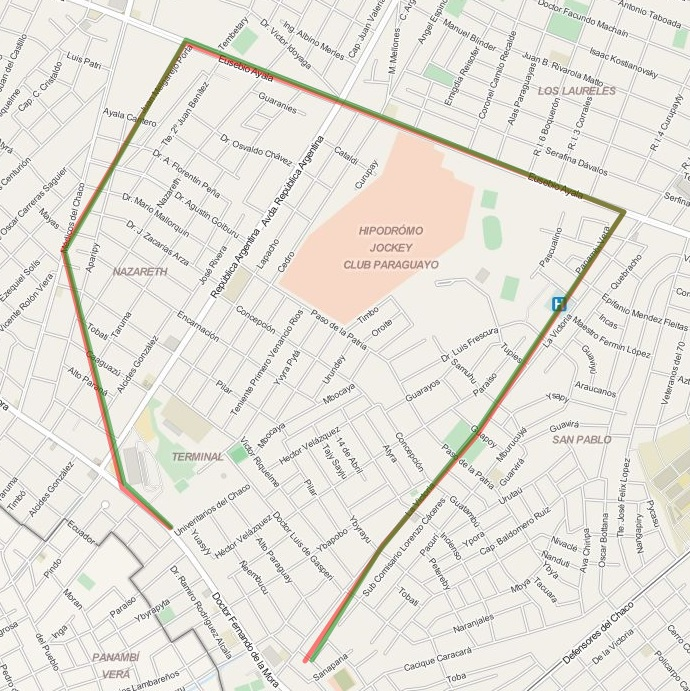
\includegraphics[width=0.7\textwidth]{capitulos/7/figuras/figura3.jpg}
	\caption{\label{fig:mm_2m} MM con intervalo de 2 minutos}	
\end{figure}

\section{Análisis de Tráfico}

Para realizar las pruebas sobre el análisis de tráfico se distribuyó la aplicación Autotracks a través de Google Play, se observan los resultados obtenidos a durante un periodo de 5 semanas de uso de la aplicación. Durante ese periodo de tiempo un promedio de 200 usuarios utilizaron la aplicación diariamente, generando un total de 123419 puntos observados desde sus dispositivos móviles.




